\documentclass[12pt,a4paper,twoside]{report}
\usepackage[italian]{babel}
\usepackage{newlfont}
\usepackage{color}
\textwidth=450pt\oddsidemargin=0pt

% INIZIO HEADER INSERITI DA ME, DA CUI HO TOLTO GLI HEADER CHE SI RIPETONO

%\documentclass[12pt,a4paper]{article}
%\usepackage[utf8]{inputenc}
\usepackage{titling}
\usepackage[backend=bibtex,
			style=numeric,
			sorting=none
			]{biblatex}
\addbibresource{bibliography.bib} %Import the bibliography file
%\setlength{\droptitle}{-2cm}% change title position
\usepackage{amsmath}
%\usepackage{amsfonts}
\usepackage{amssymb}
%\usepackage[T1]{fontenc}
%\usepackage{multirow}
%\usepackage{array}
%\newcolumntype{P}[1]{>{\centering\arraybackslash}p{#1}}
%\newcolumntype{M}[1]{>{\centering\arraybackslash}m{#1}}
\usepackage{graphicx}
\usepackage[version=4]{mhchem}
%\usepackage{siunitx}
\usepackage{float}
\usepackage[top=1.7in,left=1in,right=1in]{geometry}
%\usepackage{listings}
%\usepackage{circuitikz}
\usepackage{subcaption}
%\usepackage{tabularx}
%\renewcommand{\lstlistingname}{Code}
%\renewcommand{\lstlistlistingname}{List of Code}
%\lstdefinestyle{chstyle}{
	%	backgroundcolor=\color{gray!12},
	%	basicstyle=\ttfamily\small,
	%	commentstyle=\color{green!60!black},
	%	keywordstyle=\color{magenta},
	%	stringstyle=\color{blue!50!red},
	%	showstringspaces=false,
	%	%captionpos=b,
	%	numbers=left,
	%	numberstyle=\footnotesize\color{gray},
	%	numbersep=10pt,
	%	%stepnumber=2,
	%	tabsize=2,
	%	frame=L,
	%	framerule=1pt,
	%	rulecolor=\color{red},
	%	breaklines=true,
	%	inputpath=code
	%}
%\renewmenumacro{\directory}{pathswithfolder} % default: path
%\renewmenumacro{\keys}{shadowedroundedkeys} % default: roundedkeys
%\setlength{\arrayrulewidth}{1.0pt}
%\renewcommand{\arraystretch}{1}
\usepackage{mathcomp}

%\usepackage{fontspec}
%\setmainfont{Calibri}

\usepackage{fancyhdr}
\pagestyle{fancy}
%\renewcommand{\chaptermark}[1]{\markboth{\MakeUppercase{\chaptername\ \thechapter.\ #1}}{}}
\renewcommand{\chaptermark}[1]{\markboth{\MakeUppercase{CAP.\ \thechapter\ --\ #1}}{}}
\setlength{\headwidth}{13cm}
\fancyhead{} % clear all header fields
\fancyhead[LO]{\footnotesize \textsl{\rightmark}}
\fancyhead[RE]{\footnotesize \textsl{\leftmark}}
\fancyhead[LE,RO]{\footnotesize \thepage}
\fancyfoot{} % clear all footer fields
\renewcommand{\headrulewidth}{0.3pt}

% è già di default interlinea singola
\usepackage{setspace}

\newsavebox{\largestimage}

%\usepackage[font=it]{caption}
%\usepackage{indentfirst}

\usepackage{hyperref}
\hypersetup{
	colorlinks,
	citecolor=black,
	filecolor=black,
	linkcolor=black,
	urlcolor=black
}

% FINE HEADER INSERITI DA ME

\begin{document}
	\begin{titlepage}
		\begin{center}
			{{\Large{\textsc{Alma Mater Studiorum $\cdot$ Universit\`a di Bologna}}}} 
			\rule[0.1cm]{15.8cm}{0.1mm}
			\rule[0.5cm]{15.8cm}{0.6mm}
			\\\vspace{3mm}
			
			{\small{\bf Scuola di Scienze \\ 
					Dipartimento di Fisica e Astronomia\\
					Corso di Laurea in Fisica}}
			
		\end{center}
		
		\vspace{23mm}
		
		\begin{center}\textcolor{red}{
				%
				% INSERIRE IL TITOLO DELLA TESI
				%
				{\LARGE{\bf TITOLO TESI}}\\
		}\end{center}
		
		\vspace{50mm} \par \noindent
		
		\begin{minipage}[t]{0.47\textwidth}
			%
			% INSERIRE IL NOME DEL RELATORE CON IL RELATIVO TITOLO DI DOTTORE O PROFESSORE
			%
			{\large{\bf Relatore: \vspace{2mm}\\\textcolor{red}{
						Prof./Dott. Nome Cognome}\\\\
					%
					% INSERIRE IL NOME DEL CORRELATORE CON IL RELATIVO TITOLO DI DOTTORE O PROFESSORE
					%
					% SE NON AVETE UN CORRELATORE CANCELLATE LE PROSSIME 3 RIGHE
					%
					\textcolor{red}{
						\bf Correlatore: (eventuale)
						\vspace{2mm}\\
						Prof./Dott. Nome Cognome\\\\}}}
		\end{minipage}
		%
		\hfill
		%
		\begin{minipage}[t]{0.47\textwidth}\raggedleft {
				{\large{\bf Presentata da:
						\vspace{2mm}\\
						Simone Pasquini}}}
		\end{minipage}
		
		\vspace{40mm}
		
		\begin{center}
			Anno Accademico { 2023/2024}
		\end{center}
		
	\end{titlepage}
	\newpage
	\newgeometry{top=4cm,bottom=4cm,left=4cm,right=4cm}
	\doublespacing % Also singlespacing, onehalfspacing 
	\chapter*{Sommario}
		Questo è l'inizio del sommario.
	\newpage
	\tableofcontents
	\newpage
	\addcontentsline{toc}{chapter}{Introduzione}
	\chapter*{Introduzione}
		Questo è l'inizio dell'introduzione. metodo del SSN (sistema già attivo nella sanità+Questo percorso ha portato alla marcatura CE del centro e nel 2017 l'adroterapia è stata inserita nei Livelli Essenziali di Assistenza.
		
		 statale).https://scienzapertutti.infn.it/4-adroterapia-dalla-fisica-alla-terapia
	\newpage
	\addcontentsline{toc}{chapter}{Conclusioni}
	
	\chapter{Terapie oncologiche e radiazioni ionizzanti}
	\section{Incidenza tumorale nel mondo}
	Le neoplasie sono tra le principali cause di morte per la popolazione mondiale. Un tumore è una patologia legata al mancato funzionamento del ciclo cellulare. Le cellule tumorali, per via di mutazioni genetiche che sfuggono ai meccanismi di controllo che regolano la proliferazione cellulare, iniziano a dividersi in modo eccessivo formando delle masse anomale, chiamate tumori, che talvolta possono invadere altri tessuti dell'organismo ostacolandone le funzioni vitali, in un processo chiamato metastasi. In quest'ultimo caso si parla di tumore maligno o cancro.
		
	Attualmente, è possibile prevenire fino al $50\%$ di tumori evitando fattori di rischio e implementando strategie di prevenzione già esistenti (cita
	%https://www.who.int/news-room/fact-sheets/detail/c+ancer
	), anche se ciò dipende dalla tempestività delle diagnosi, dalla tipologia delle cure e dal tipo di tumore. Si stima che nei Paesi industrializzati,\footnote{Si fa riferimento ai Paesi OCSE (Organizzazione per la Cooperazione e lo Sviluppo Economico).} nel $2021$, il cancro è la seconda causa di morte (causando il $21\%$ dei decessi totali), preceduto dalle malattie cardiovascolari (cita %https://www.oecd-ilibrary.org/docserver/7a7afb35-en.pdf?expires=1709230714&id=id&accname=guest&checksum=FBEABF3EDA6F2040465BB27356B8D68B
	). Sebbene il tasso di mortalità sia sceso sin dal $2000$, a livello mondiale il numero di casi diagnosticati di cancro (nel $2022$) attesta a quasi $20.0$ milioni\footnote{Negli ultimi dieci anni il numero di casi di tumore è aumentato di anno in anno, soprattutto a causa dell'invecchiamento progressivo della popolazione (cita
	%https://www.iss.it/-/tumori-in-aumento-le-diagnosi-in-europa-anche-per-effetto-dell-invecchiamento-demografico
	), ma nel biennio $2020$-$2021$ il trend è cambiato a causa della pandemia di COVID-$19$, che ha precluso l'accesso a screening oncologici (nel periodo gennaio--ottobre $2020$ vi è stato un calo del $37.3\%$ di test diagnostici rispetto al periodo pre-pandemico) (cita
	%https://www.ncbi.nlm.nih.gov/pmc/articles/PMC9807424/
	). Ciò potrebbe rivelarsi fatale nel medio-lungo termine causando un aumento dei tassi di incidenza e mortalità (cita
	%https://doi.org/10.1787/ae3016b9-en
	).} (pari al $2.5\tcperthousand$ della popolazione totale (citare %https://data.unicef.org/resources/data_explorer/unicef_f/?ag=UNICEF&df=GLOBAL_DATAFLOW&ver=1.0&dq=WORLD.DM_POP_TOT.&startPeriod=2022&endPeriod=2022
	)), di cui il $48.8\%$ hanno portato alla morte del paziente (citare
	%https://gco.iarc.who.int/en
	). Inoltre, i tassi di mortalità dovuti alle patologie tumorali sono strettamente dipendenti dall'indice di sviluppo dei Paesi (ISU), infatti da un tasso di mortalità del $39.2\%$ dei Paesi con ISU molto alto, si sale sino al $67.1\%$ dei Paesi con basso ISU (cita
	%https://gco.iarc.who.int/today/en/dataviz/bars?mode=population&key=total&group_populations=0&types=0_1&sort_by=value1&populations=900_981_982_983_984&multiple_populations=1&values_position=out&cancers_h=39&include_nmsc=1&age_end=17
	).
	
	Altri fattori rendono i tassi di incidenza e mortalità per patologie tumorali ulteriormente disuniformi, quali il sesso e l'età. A livello globale, l'incidenza di cancro negli uomini è più alta rispetto a quella delle donne dell'$8.0\%$ (cita
	%https://gco.iarc.who.int/media/globocan/factsheets/cancers/39-all-cancers-fact-sheet.pdf
	), dovuta anche al fatto che i primi si espongono maggiormente a fattori di rischio quali fumo e consumo di alcol. Inoltre, il $58\%$ di tumori viene diagnosticato nelle persone con più di 65 anni (cita
	%https://www.cdc.gov/cancer/uscs/about/data-briefs/no29-USCS-highlights-2019-incidence.htm
	).
	
	Sebbene i dati sopra citati testimonino la gravità delle patologie oncologiche, è indubbio che il progresso della scienza degli ultimi anni abbia permesso un notevole sviluppo nell'efficacia dei trattamenti oncologici: nel decennio $2010$--$2020$, il numero di persone che sopravvive dopo una diagnosi di cancro aumenta approssimativamente del $3\%$ in Paesi come l'Italia, gli Stati Uniti d'America, il Regno Unito e la Svizzera (cita
	%https://www.ncbi.nlm.nih.gov/pmc/articles/PMC5807846/pdf/12885_2018_Article_4053.pdf
	).
	
	\section{Terapie oncologiche}
	Il trattamento di un tumore avviene in molti modi differenti e varia in base al tipo di cancro, il suo stadio di avanzamento e dagli obiettivi che si intendono raggiungere al termine dei trattamenti. Oggigiorno, le terapie oncologiche si distinguono in locali (o regionali) e generali (o sistemiche), in base all'estensione del tumore che colpisce il paziente. Al primo gruppo appartengono terapie come la chirurgia, la radioterapia e l'adroterapia, mentre al secondo afferiscono la chemioterapia e l'immunoterapia. Tali tecniche, proprio per la loro diversità, sono spesso utilizzate in maniera complementare per aumentare l'efficacia dei trattamenti clinici. Per pianificare il trattamento più adeguato al fronte di una certa patologia oncologica, si introduce il concetto di stadiazione, che è un modo di descrivere in maniera schematica, rigorosa e standardizzata la grandezza di un tumore e la sua diffusione al di fuori della sede originale (cita
	%https://www.airc.it/cancro/affronta-la-malattia/la-fase-della-diagnosi/stadiazione
	). Le informazioni tipiche della stadiazione includono la collocazione del tumore, la sua estensione e se si è diffuso in parti del corpo differenti. Infatti, come già accennato, le cellule tumorali si moltiplicano in modo incontrollato andando a occupare (per mezzo del sistema linfatico o sanguigno) organi e tessuti distanti dalla sede di sviluppo originaria, attraverso un fenomeno chiamato metastatizzazione. Chiaramente, ciascuna terapia possiede effetti collaterali correlati all'azione distruttiva che si impiega per debellare la malattia oncologica.
	
	Se il tumore ha raggiunto un'estensione tale da formare metastasi, si scelgono trattamenti sistemici in modo che si possa debellare o, quantomeno, contenere la malattia oncologica. La chemioterapia consiste nella somministrazione di uno o più farmaci citotossici (o antiblastici) capaci di aggredire le cellule cancerose (cita
	%https://www.aimac.it/libretti-tumore/chemioterapia/che-cos-e-la-chemioterapia
	), mentre nell'immunoterapia si tenta di istruire il sistema immunitario affinché riconosca ed elimini gli oncogeni, i geni modificati che causano il cancro.
	
	Qualora il tumore fosse localizzato, ben raggiungibile dall'esterno e sufficientemente lontano da organi vitali, si ricorre a operazioni chirurgiche, con le quali si asporta la massa tumorale dal corpo del paziente. Prima o dopo l'operazione chirurgica, si procede con tecniche radioterapiche, adroterapiche o chemioterapiche in base alle necessità. Ad esempio, nella radioterapia neoadiuvante il trattamento radioterapico viene effettuato prima dell'intervento chirurgico, mentre nella radiochemioterapia concomitante si eseguono sessioni di chemioterapia e radioterapia a seguito dell'operazione chirurgica (cita
	%https://www.aimac.it/libretti-tumore//perche-si-attua-la-radioterapia
	). In generale, la commistione di suddette tecniche consente di rimuovere tracce di cellule tumorali, evitandone eventuali proliferazioni successive.
	
	Nel caso in la massa tumorale non sia rimovibile attraverso un'operazione chirurgica a causa della sua localizzazione anatomica (è il caso di neoplasie legate a organi la cui rimozione sarebbe troppo invalidante per il paziente (cita
	%https://web.infn.it/foot/
	)), si preferisce ricorrere alla radioterapia e all'adroterapia, ove quest'ultima è una forma avanzata di radioterapia. Pur non essendo invasive come la chirurgia, tali tecniche permettono di danneggiare specifici tessuti biologici malati utilizzando radiazione ionizzante, composta da fasci di fotoni ed elettroni in radioterapia e da particelle adroniche (come protoni, neutroni e ioni) in adroterapia (si veda \hyperref[fig:simulation]{Fig. 1.1}). In particolare, lo scopo di entrambi i trattamenti è quello di depositare una quantità di energia (detta "dose") capace di provocare un danno biologico tale da inibire la crescita del tumore con effetti collaterali minimi (cita
	%rivista asimmetrie, DOI 10.23801/asimmetrie.2023.35.03
	). Sebbene sembrino molto simili, la radioterapia e l'adroterapia presentano caratteristiche fisiche e radiobiologiche molto differenti, i cui dettagli verranno evidenziati nel prosieguo. Mentre un fascio radioterapico rilascia la dose in una regione piuttosto ampia, aumentando il rischio di distruggere cellule sane situate prima e dopo il tumore, le particelle adroniche irradiano una grande quantità di energia in uno spazio molto limitato, attraverso il caratteristico picco di Bragg. Pertanto, visto che l'adroterapia permette di definire in modo molto più preciso la regione da irradiare (cita
	%https://web.infn.it/foot/
	), il suo obiettivo non è solo quello di distruggere più efficacemente porzioni di cellule tumorali, ma anche quello di minimizzare i danni a carico dei tessuti sani circostanti (cita
	%https://fondazionecnao.it/adroterapia/cos-e-l-adroterapia
	), al fine di qualità della vita del paziente.
	
	\begin{figure}[H]
		\centering
		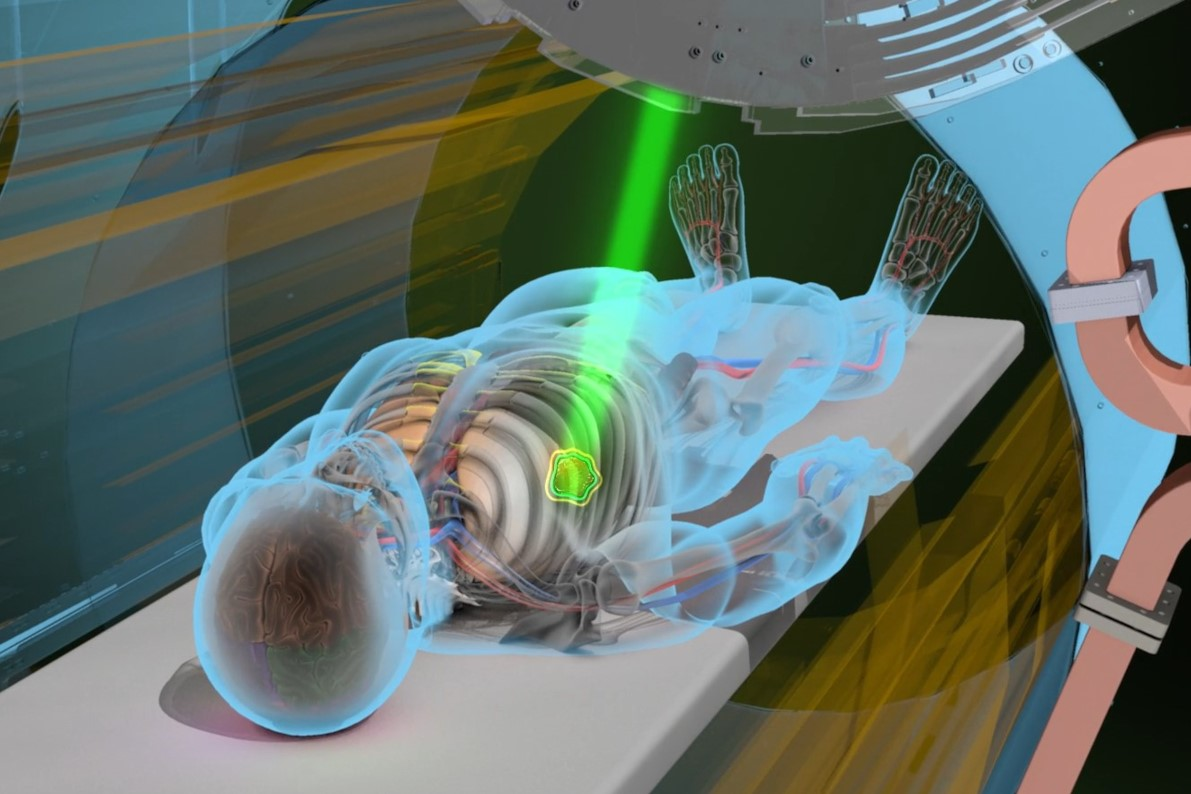
\includegraphics[width=0.9\linewidth]{images/simulation.jpg}
		\caption{Simulazione di un irraggiamento radioterapico o adroterapico sul corpo di un paziente (cita
			%https://www.youtube.com/watch?v=Uu261OEf3Pg
			).}
		\label{fig:simulation}
	\end{figure}
	
	Sebbene l'adroterapia sia complessivamente più efficace rispetto alla radioterapia nella distruzione di cellule tumorali e nella salvaguardia dei tessuti sani, è un trattamento relativamente recente (si veda \hyperref[storia_adroterapia]{Sez. ??}) che ha bisogno, tra le varie e complesse strutture, di acceleratori di particelle; ciò rende l'adroterapia meno sviluppata e più costosa della radioterapia. Inoltre, oggi non esiste una teoria analitica che sia in grado di spiegare i processi nucleari che intercorrono tra le particelle adroniche e i nuclei del corpo umano (cita
	%FOOT CDR
	), quindi, prima di poter applicare trattamenti medici efficaci e sicuri, si rendono necessarie numerosissime misure sperimentali (una buona parte delle quali sono tuttora fornite dall'esperimento FOOT) in grado di colmare tali lacune (cita
	%https://web.infn.it/foot/
	). Per questo motivo, il settore di ricerca adroterapico è molto attivo e coinvolge un crogiolo culturale di fisici, medici, biologi che studiano gli effetti della frammentazione nucleare sulle cellule umane, analizzabili solo mediante un approccio interdisciplinare.
	
	L'adroterapia, però, non appartiene esclusivamente all'ambito della sperimentazione, ma costituisce una realtà interazionale nella cura dei tumori a tutti gli effetti. Infatti, alla fine del $2023$ quasi $410000$ pazienti hanno effettuato trattamenti adroterapici a livello globale (di cui $350000$ con protoni, $56000$ con ioni carbonio e $3500$ con elio, pioni e altre particelle), un numero tre volte maggiore di quello emerso a fine $2014$ (cita
	%https://ptcog.site/
	). Pur essendo tali numeri incoraggianti, è necessario continuare a investire risorse nella ricerca in modo che esperimenti della caratura di FOOT possano rendere l'adroterapia un trattamento più diffuso e accessibile a tutti.
	

	\section{Storia della radioterapia}
	La storia della radioterapia inizia nel novembre del $1895$ con un episodio di serendipità, il cui protagonista è il fisico tedesco Wilhelm C. von Röntgen, scopritore dei raggi X. Durante lo studio dei raggi catodici prodotti da un tubo di Crookes, Röntgen si accorse che della radiazione sconosciuta (denominata da lui stesso "X", poiché incognita sino ad allora) oltrepassava la lastra di vetro che ricopre lo strumento. Röntgen comprese sin da allora le grandi potenzialità dei neonati raggi X, utilizzabili per proiettare su uno schermo il materiale che attraversano delineandone le specificità. Fu proprio il fisico a effettuare la prima radiografia alla mano di sua moglie (\hyperref[fig:rongten]{Fig. 1.2}), esponendo tuttavia quest'ultima a non pochi rischi, essendo i raggi X un tipo di radiazione ionizzante.\footnote{Una radiazione si dice ionizzante quando ha energia sufficiente a liberare gli elettroni legati agli atomi della materia in cui penetra. Per questo motivo la radiazione ionizzante è capace di provocare danni biologici ai tessuti del corpo umano.} Le immediate applicazioni della scoperta di Röntgen in campo medico gli valsero il premio Nobel per la fisica nel $1901$(cita
	%https://www.nobelprize.org/prizes/physics/1901/rontgen/facts/
	).
	
	\begin{figure}[H]
		\centering
		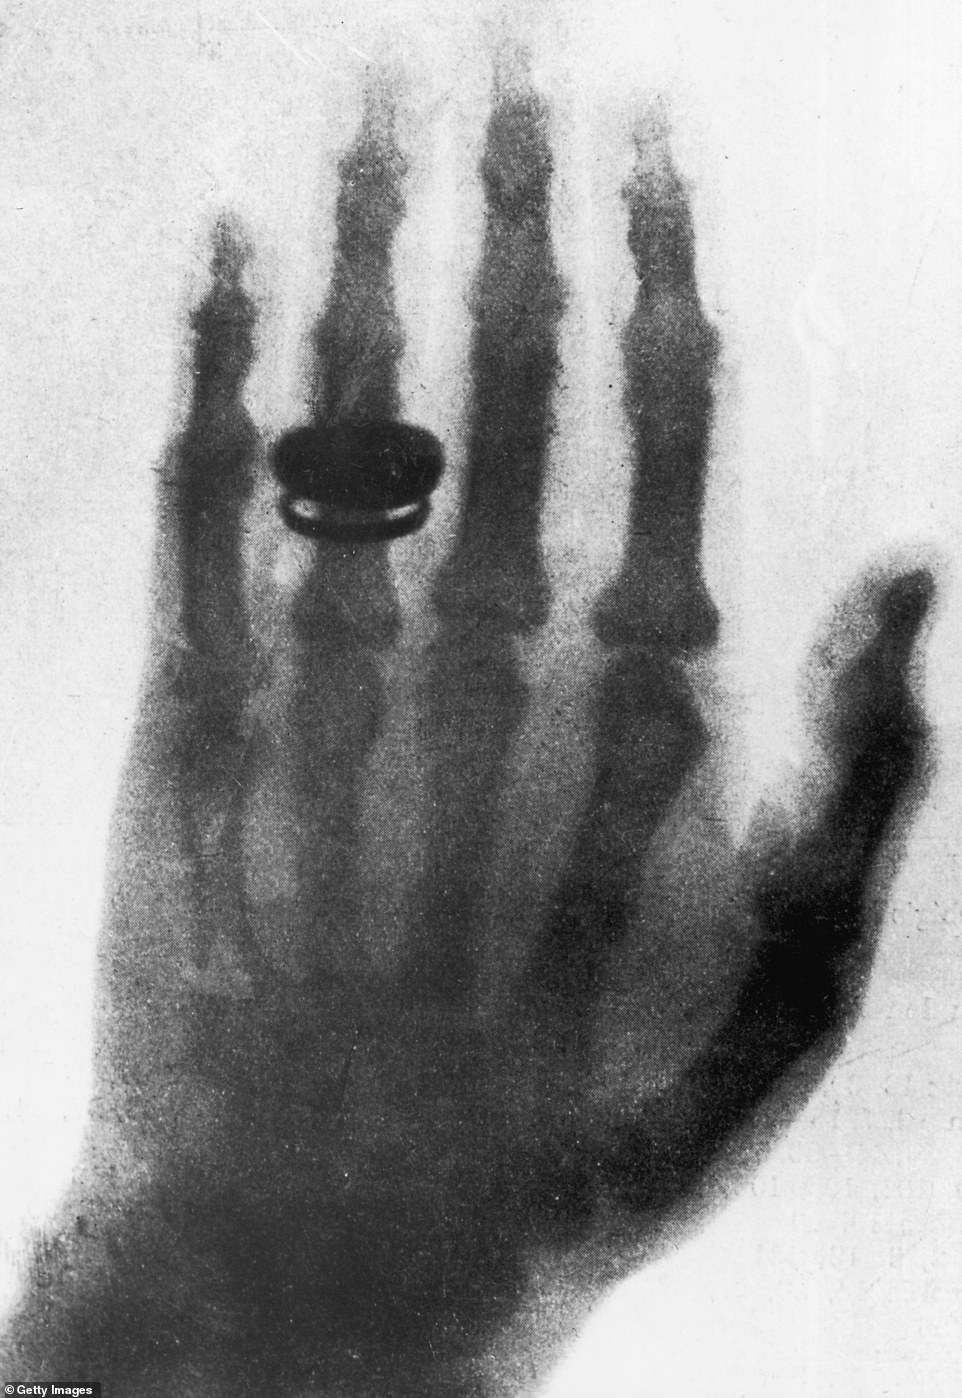
\includegraphics[width=0.5\linewidth]{images/rongten.jpg}
		\caption{La prima lastra a raggi X della mano di Anna Bertha Ludwig, moglie di Ron, dopo 15 minuti di esposizione (cita
			%https://www.dailymail.co.uk/news/article-6491287/Roentgens-human-X-ray-wifes-hand-1895.html
			).}
		\label{fig:rongten}
	\end{figure}
	
	Solamente un anno dopo la scoperta di Röntgen, Antoine H. Becquerel, studiando la fosforescenza dei sali di uranio, notò che alcuni materiali emettevano raggi elettromagnetici senza essere eccitati dalla luce solare. Becquerel scoprì così la radioattività spontanea dell'uranio che gli valse il premio Nobel per la fisica nel $1903$ condiviso con i coniugi Pierre Curie e Maria Sklodowska per la scoperta del radio \ce{^{226}_{88}Ra}. Da quel momento in avanti, la sperimentazione degli effetti terapeutici dei raggi X e della radioterapia portò a svariati successi, per esempio legati alla cura del \textit{lupus vulgaris} e del \textit{lupus eritematoso}.
	
	\subsection{Storia dell'adroterapia}\label{storia_adroterapia}
	
	L'avvento delle due Guerre Mondiali da un lato rallentò il progresso della comunità scientifica, dall'altro rappresentò un'occasione utile ai popoli per sfoggiare il proprio avanzamento tecnico-scientifico perché, riportando una sciagurata dichiarazione del "generale in camice bianco" Fritz Haber, la scienza "serve all’umanità in pace e alla patria in guerra"(cita
	%James, Steinhauser, Hoffmann, Friedrich OneHundredYearsOfChemicalWarfare
	). In particolare, la corsa agli armamenti atomici favorì un forte sviluppo della teoria atomica e nucleare, la cui conoscenza approfondita fu sfruttata inizialmente come arma e poi come risorsa, impiegabile ad esempio nella cura di malattie. Un caso esemplare della dicotomia scientifica di quegli anni è rappresentato da Robert R. Wilson che dopo aver lavorato ai laboratori di Los Alamos per il Progetto Manhattan\footnote{Il progetto Manhattan fu un programma di ricerca attivo dal $1942$ al $1946$ per la produzione della prima arma nucleare. Viene tragicamente ricordato per la costruzione degli ordigni \textit{Little Boy} e \textit{Fat Man} con cui furono bombardate rispettivamente Hiroshima e Nagasaki.} propose per primo l'utilizzo di protoni come terapia oncologica bel $1946$ notandone le potenzialità rispetto alla radioterapia convenzionale (cita
	%https://inspirehep.net/files/d86d8a0dc5736a2298f58f84efc8dc81
	) e nel $1967$ fondò il Fermilab, uno dei maggiori centri di ricerca per la fisica delle particelle elementari. Wilson, misurando la dose rilasciata dai fasci di protoni prodotti dal ciclotrone dei Lawrence Berkeley National Laboratory (LBL), notò l'efficienza superiore del picco di Bragg protonico rispetto alla radioterapia convenzionale. Nel suo articolo (cita
	%https://inspirehep.net/files/d86d8a0dc5736a2298f58f84efc8dc81, ripetizione
	), lo scienziato fa anche rifermento a un possibile uso futuro degli ioni più pesanti, come gli ioni di carbonio, che "potrebbero diventare terapeuticamente pratici". Infatti, nel $1954$, nei LBL fu trattato il primo paziente con i protoni, a cui seguirono i primi trattamenti con elio nel $1957$ e con ioni di neon nel $1975$ (cita
	%https://indico.cern.ch/event/24728/attachments/424989/590019/RIVISTA_MEDICA_2008-14_1.pdf
	). Si sottolinea che in questi primi trattamenti, e in una buona parte dei successivi, le particelle venivano collimate senza sfruttare la loro carica elettrica, proprietà che sarebbe diventata fondamentale per la loro detezione e per il loro controllo attraverso campi magnetici. Un grande sviluppo della terapia protonica ci fu con la costruzione del ciclotrone di Harvard del $1949$ (in sostituzione del ciclotrone del $1937$ trasferito a Los Alamos per il Progetto Manhattan (cita
	%https://cerncourier.com/a/synchrocyclotron-survivor-to-bow-out-after-50-years/
	)) col quale si ottennero numerosi successi, specialmente per il melanoma oculare e per i tumori ossei della base del cranio, che convinsero in molti sulla superiorità dei protoni rispetto ai raggi X per i tumori vicini agli organi a rischio (cita
	%Wilson R.: A brief history of the Harvard University Cyclotron. Harvard University Press, 2003.
	).
	
	Gli studi del ciclotrone di Harvard spinsero anche i laboratori russi e giapponesi ad avviare programmi di ricerca nella terapia adronica. Di particolare importanza è l'apertura del centro HIMAC (Heavy Ion Medical Accelerator in Chiba, si veda \hyperref[fig:himac]{Fig. 1.3}) (cita
	%Hirao Y., Ogawa H. et al.: Heavy ion synchrotron for medical use. Nucl Phys 1992; A 538: 541c-550c.
	) a Chiba (Giappone) che, nel $1994$, trattò per primo un paziente con un fascio di ioni carbonio, il cui rilascio di dose è nettamente superiore a quello di fotoni e protoni ed è per questo più efficace nel controllo di tumori radioresistenti e di neoplasie più comuni (per esempio ai polmoni o al fegato).
	
	\begin{figure}[H]
		\centering
		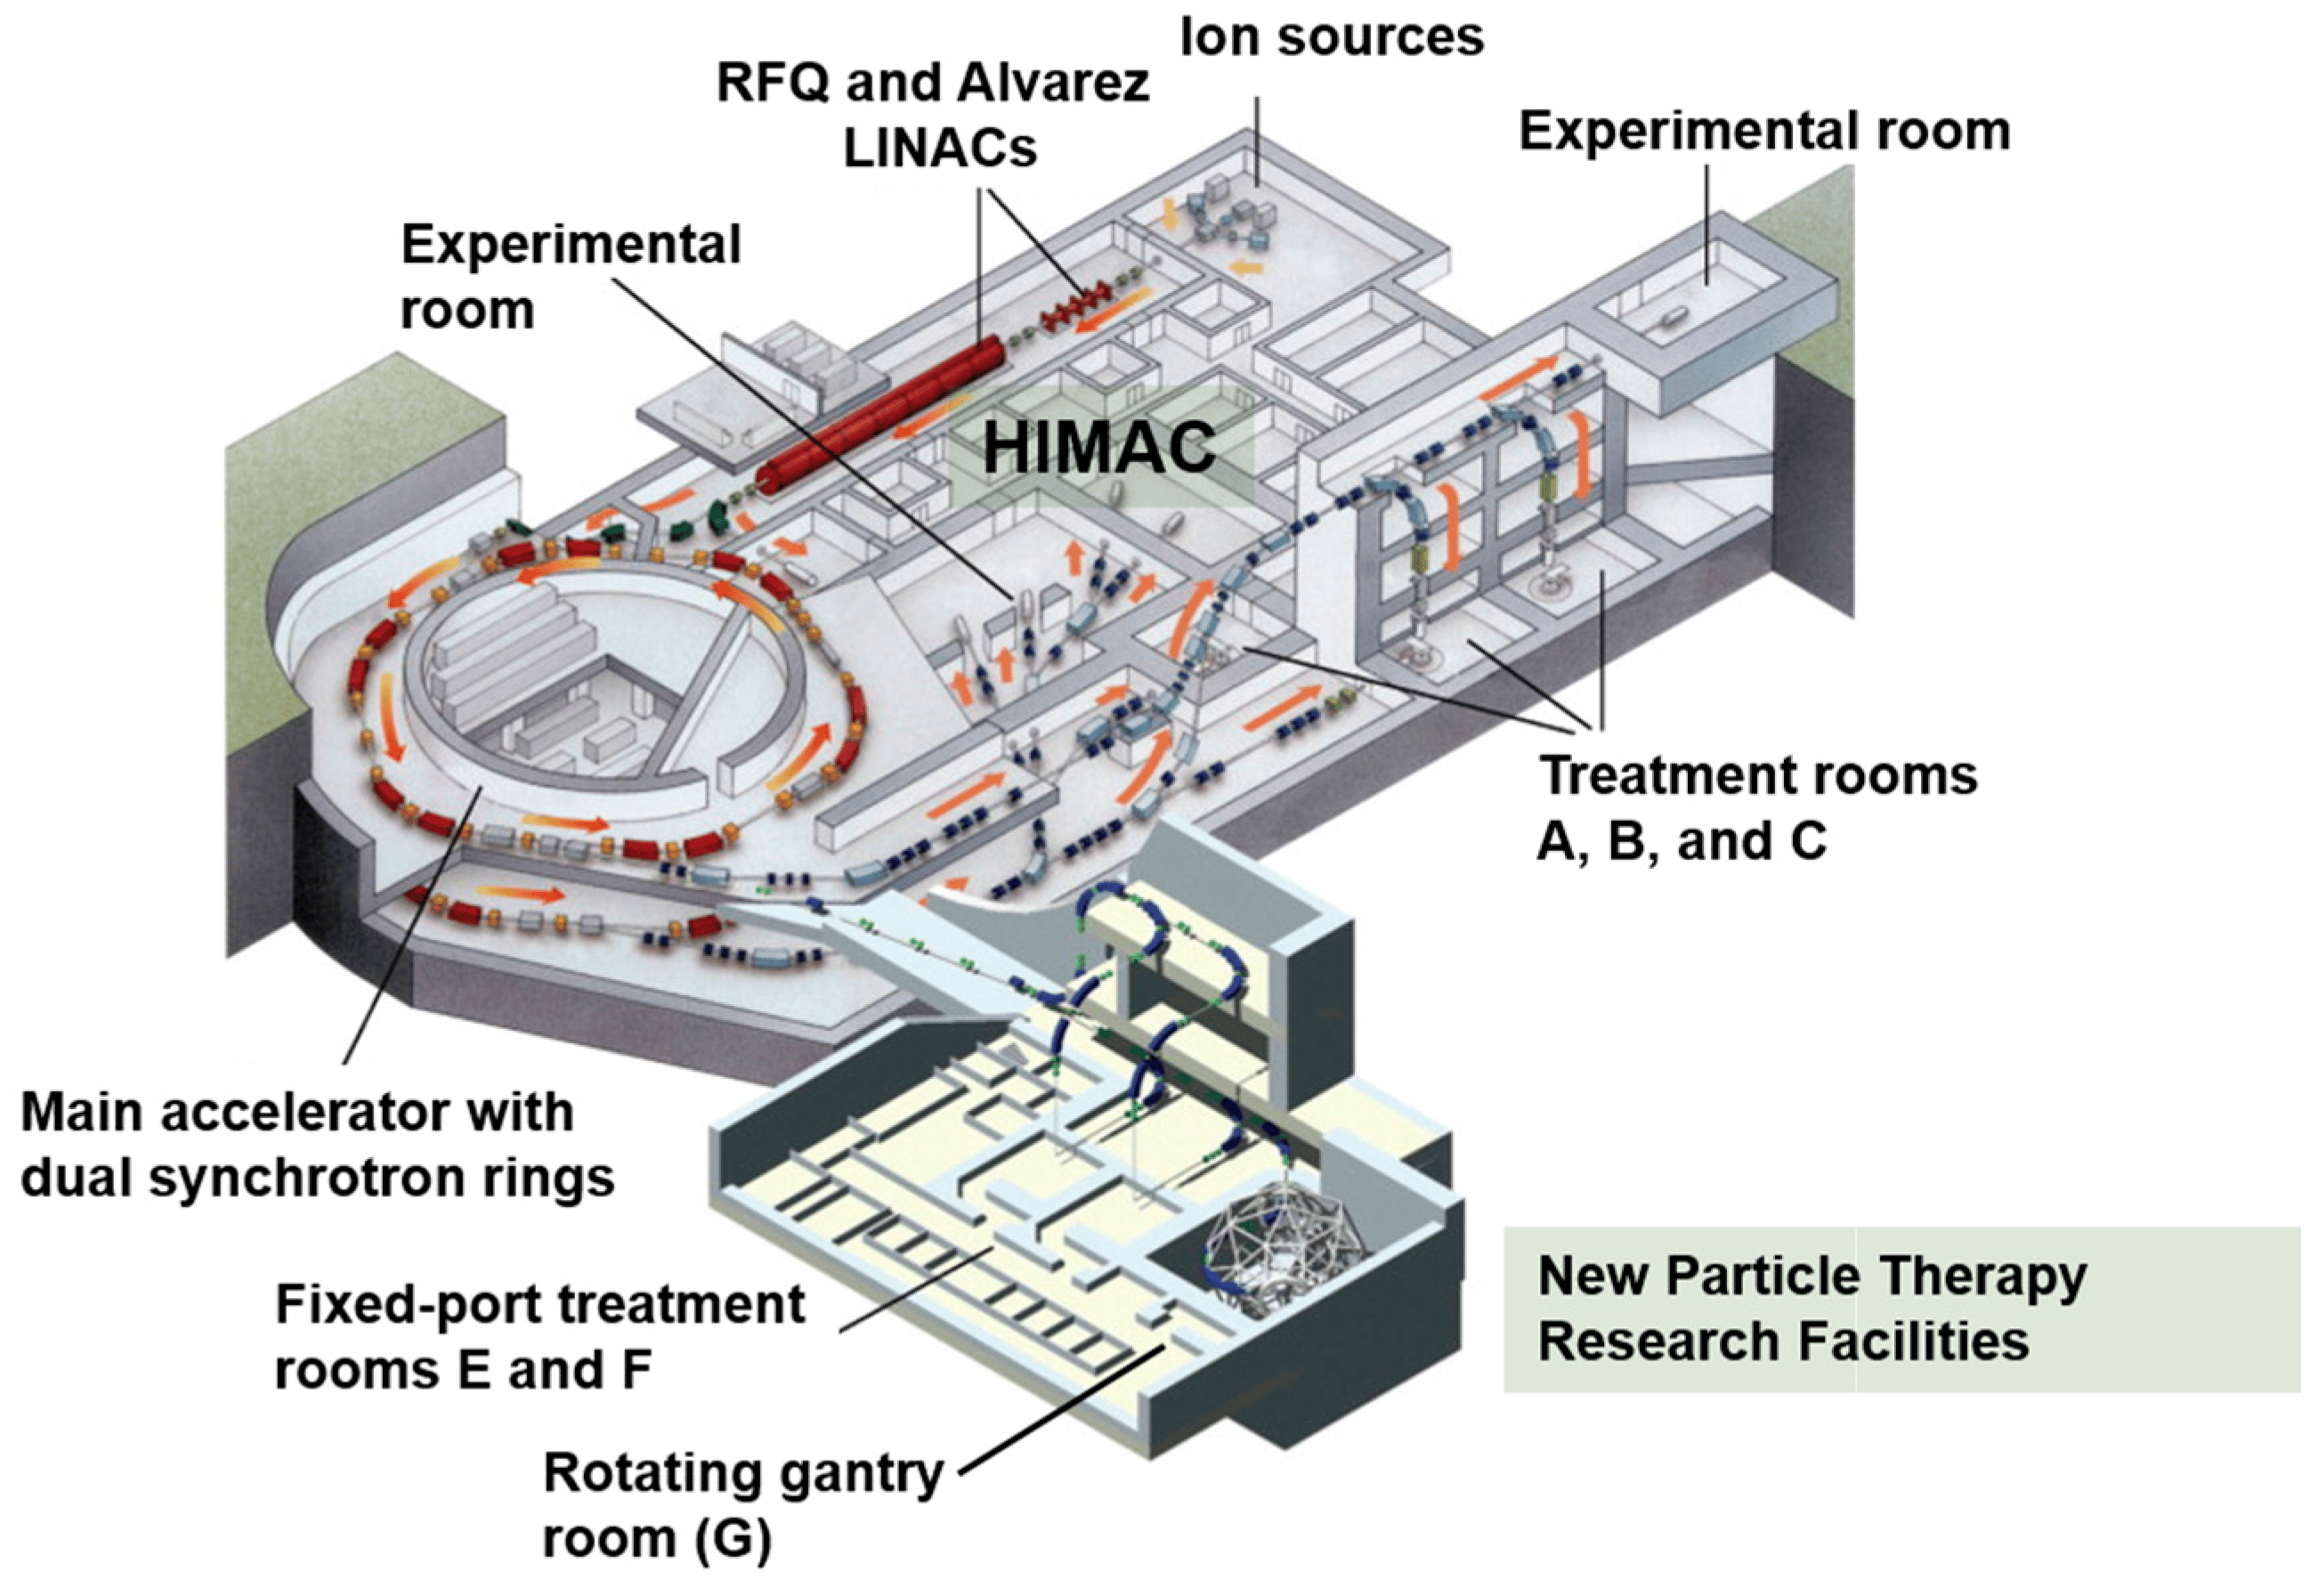
\includegraphics[width=0.9\linewidth]{images/himac.png}
		\caption{Panoramica delle strutture di ricerca HIMAC presso l'Istituto Nazionale di Scienze Radiologiche a Chiba (cita
			%https://www.mdpi.com/2072-6694/10/3/66
			).}
		\label{fig:himac}
	\end{figure}
	
	La prima iniziativa completamente europea di un centro terapico agli ioni arrivò solo nel $1987$ con EULIMA (EUropean Light Ion Medical Accelerator). Il progetto prevedeva la costruzione di un sincrotrone\footnote{I ciclotroni, con diametro di circa $5\mbox{ m}$, si utilizzano per produrre fasci di protoni, mentre i sincrotroni, con diametro di oltre $10\mbox{ m}$, si usano principalmente per generare ioni carbonio (cita
		%rivista asimmetrie, DOI 10.23801/asimmetrie.2023.35.03
	).} che, purtroppo, non fu mai costruito; si dovettero attendere progetti esclusivamente nazionali per un decisivo cambio di passo della terapia agli ioni, soprattutto nel decennio $1994$--$2004$, in cui iniziò la costruzione di due centri fondamentali per i trattamenti con protoni e ioni carbonio. Il primo è l'Heidelberg Ionenstrahl Therapy (HIT), aperto a Heidelberg (Germania) nel 2009, il secondo, italiano, è il Centro Nazionale di Adroterapia Oncologica (CNAO) di Pavia, attivo sin dal 2011 (cita
	%https://indico.cern.ch/event/24728/attachments/424989/590019/RIVISTA_MEDICA_2008-14_1.pdf ripetizione
	).
	
	\subsection{Adroterapia in Italia}
	Una delle figure più importanti per lo sviluppo dell'adroterapia in Italia è sicuramente il fisico italiano Ugo Amaldi. La sua lungimiranza ha portato l'Italia a essere la seconda nazione europea ad avere un centro adroterapico (il CNAO) capace di effettuare trattamenti con protoni e ioni carbonio (si pensi che attualmente ne esistono solo sei in tutto il mondo (cita
	%rivista asimmetrie, DOI 10.23801/asimmetrie.2023.35.03
	)). Nei paragrafi successivi si ripercorrono le principali tappe della storia dell'adroterapia in Italia.
	
	Nel $1991$, assieme al fisico medico Giampiero Tosi, Amaldi scrisse un articolo pionieristico in cui si proponeva un centro nazionale di terapia con particelle (cita
	%Amaldi U., Tosi G.: Per un centro di teleterapia con adroni. TERA 91/2, gen 2.
	), idea accolta con entusiasmo dal noto oncologo Umberto Veronesi e dall'allora Presidente dell'Istituto Nazionale di Fisica Nucleare (INFN) Nicola Cabibbo. Un anno dopo, fu istituita la fondazione TERA (TErapia con Radiazioni Adroniche) con il duplice scopo di dare impiego a fisici e ingegneri interessati al progetto e di costruire centri adroterapici in Italia ed Europa (cita
	%https://indico.cern.ch/event/24728/attachments/424989/590019/RIVISTA_MEDICA_2008-14_1.pdf ripetizione
	).
	
	Alla fine del $1995$ si decise finalmente di creare una struttura protonterapica ai Laboratori Nazionali del Sud (LNS), sfruttando il ciclotrone superconduttore già attivo nei LNS. Il progetto, chiamato CATANA (Centro di AdroTerapia ed Applicazioni Avanzate), prevedeva la collaborazione di INFN-LNS, Dipartimento di Fisica, Istituto di Oftalmologia e Radiologia dell'Università di Catania e il Centro Siciliano di Fisica Nucleare. Il ciclotrone catanese (\hyperref[fig:catana1]{Fig. 1.4a}), dotato di un complesso sistema dosimetrico in grado di misurare la dose entro un errore del $3\%$, accelerava fasci protonici a un'energia massima di $62 \mbox{ MeV}$, range adatto soprattutto per i tumori oculari (\hyperref[fig:catana2]{Fig. 1.4b}). Nel $2002$ si trattò il primo paziente affetto da melanoma uveale e da allora oltre $500$ pazienti hanno ricevuto trattamenti con successo per tumori intraoculari, melanomi congiuntivali e linfomi non Hodgkin.\footnote{I dati del $2014$, su un numero totale di $293$ pazienti, attestano un tasso di sopravvivenza del $98\%$ (cita
	%https://agenda.infn.it/event/8475/contributions/73755/attachments/53706/63315/1.Frascaticuttone.pdf
	), percentuale pur sempre comparabile con la terapia chirurgica e fotonica, sebbene queste ultime compromettano maggiormente la capacità visiva essendo statisticamente più invalidanti dell'adroterapia.}
	
	\begin{figure}[H]
		\centering
		\savebox{\largestimage}{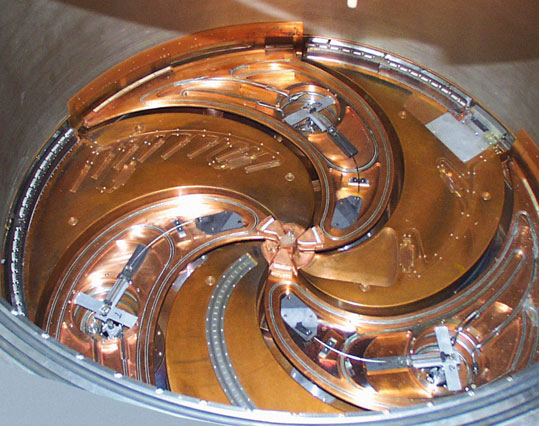
\includegraphics[width=0.49\textwidth]{images/catana1.jpg}}
		\begin{subfigure}[b]{0.49\textwidth}
			\centering
			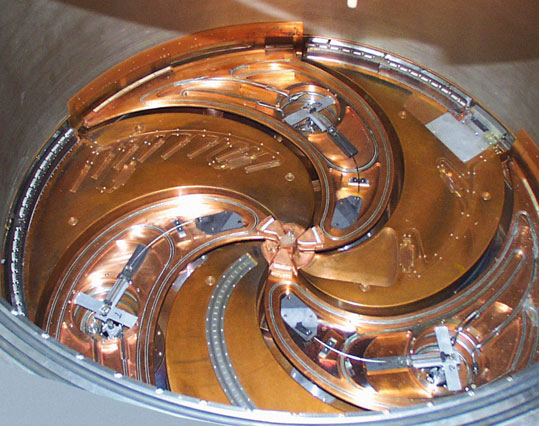
\includegraphics[width=\textwidth, scale=0.5]{images/catana1.jpg}
			\caption{Particolare interno del ciclotrone del CATANA (cita
				%rivista asimmetrie n.6 gli acceleratori
				).}
			\label{fig:catana1}
		\end{subfigure}
		\hfill
		\begin{subfigure}[b]{0.49\textwidth}
			\centering
			\raisebox{\dimexpr.5\ht\largestimage-.5\height}{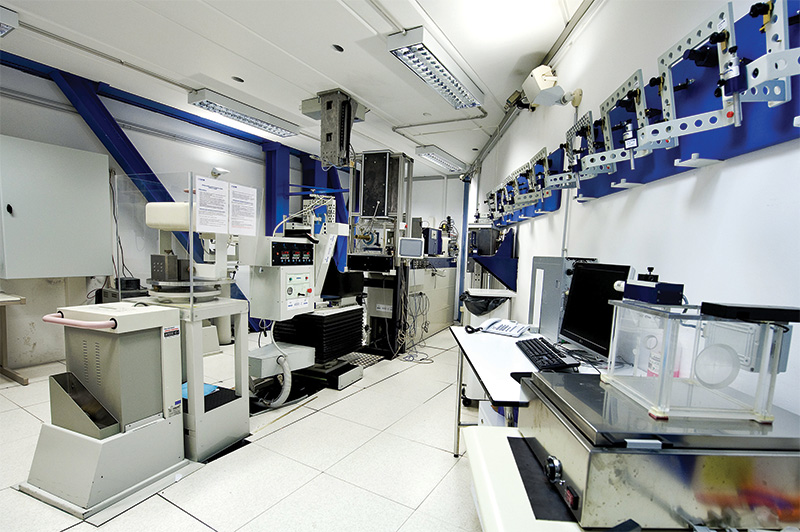
\includegraphics[width=\textwidth, scale=0.45]{images/catana2.jpg}}
			\caption{Attrezzatura presso la sala di trattamento del CATANA (cita
				%rivista asimmetrie, DOI: 10.23801/asimmetrie.2023.35.01
				).}
			\label{fig:catana2}
		\end{subfigure}
		\caption{Immagini relative al CATANA dei LNS, primo centro di protonterpia in Italia.}
		\label{fig:catana}
	\end{figure}
	
	Nel $1995$ Ugo Amaldi, con l'aiuto di Mainard Regler del progetto adroterapico austriaco Med-Austron, propose al direttivo del CERN (Conseil Européen pour la Recherche Nucléaire) di dare vita a PIMMS (Proton Ion Medical Machine Study) per la progettazione di un sincrotrone ottimizzato per il trattamento di tumori profondi attraverso ioni carbonio, protoni e altri ioni leggeri. PIMMS durò solo dal $1996$ al $2000$ ma fu un progetto talmente paradigmatico che, dopo ottimizzazioni successive, fornì una versione più compatta in termini di spazi e costi denominata PIMMS/TERA evolutasi nella versione CNAO definitivamente realizzata a Pavia (cita
	%https://fondazionecnao.it/storia
	). Proprio nel $2000$ il neoministro della Salute Umberto Veronesi autorizzò il finanziamento per la realizzazione del Centro Nazionale di Adroterapia (CNAO) e, nel maggio $2001$, istituì la Fondazione CNAO (cita
	%https://www.fondazioneveronesi.it/magazine/articoli/oncologia/potenzialita-e-limiti-delladroterapia
	). Dopo una prima fase di costruzione che ha coinvolto ben $500$ aziende italiane, Istituti ed Enti di Ricerca nazionali e internazionali, il CNAO si è attivato ufficialmente nel $2011$ (\hyperref[fig:edificio_cnao]{Fig. 1.5a}). La terapia adroterapica del CNAO, come già accennato, avviene accelerando protoni e ioni carbonio rispettivamente fino a un'energia cinetica di $250 \mbox{ MeV}$ e $4800\mbox{ MeV}$ (circa $400\mbox{ MeV/u}$\footnote{$\mbox{ MeV/u}$ è l'unità di misura dell'energia per unità di massa atomica.}). I trattamenti si svolgono in tre sale, due delle quali richiedono un fascio orizzontale mentre la terza consente un irraggiamento sia orizzontale che verticale (\hyperref[fig:sala_cnao]{Fig. 1.5b}). Protoni e ioni carbonio vengono accelerati a circa $30000\mbox{km/s}$ da un sincrotrone a forma di anello avente $25\mbox{ m}$ di diametro e $80\mbox{ m}$ di circonferenza (\hyperref[fig:sincrotrone_cnao]{Fig. 1.5c}). Gli attuali obiettivi del CNAO non sono solo quelli di arrivare a trattare circa $700$ pazienti all’anno, ma anche di diventare l’unico centro di adroterapia al mondo a disporre di protoni, ioni carbonio, altre specie ioniche e BNCT (Boron Neutron Capture Therapy) ?aggiungere riferimento alla BNCT? (cita
	https://fondazionecnao.it/futuro-scopri-progetto-espansione-cnao/gianluca-vago
	).
	
	\begin{figure}[H]
		\centering
		\subfloat[Edificio sanitario del complesso edilizio del CNAO contenente servizi sanitari, amministrativi e di alta tecnologia come il sincrotrone (cita
		%https://www.bimportale.com/cnao-centro-nazionale-adroterapia-oncologica/
		).]{\label{fig:edificio_cnao}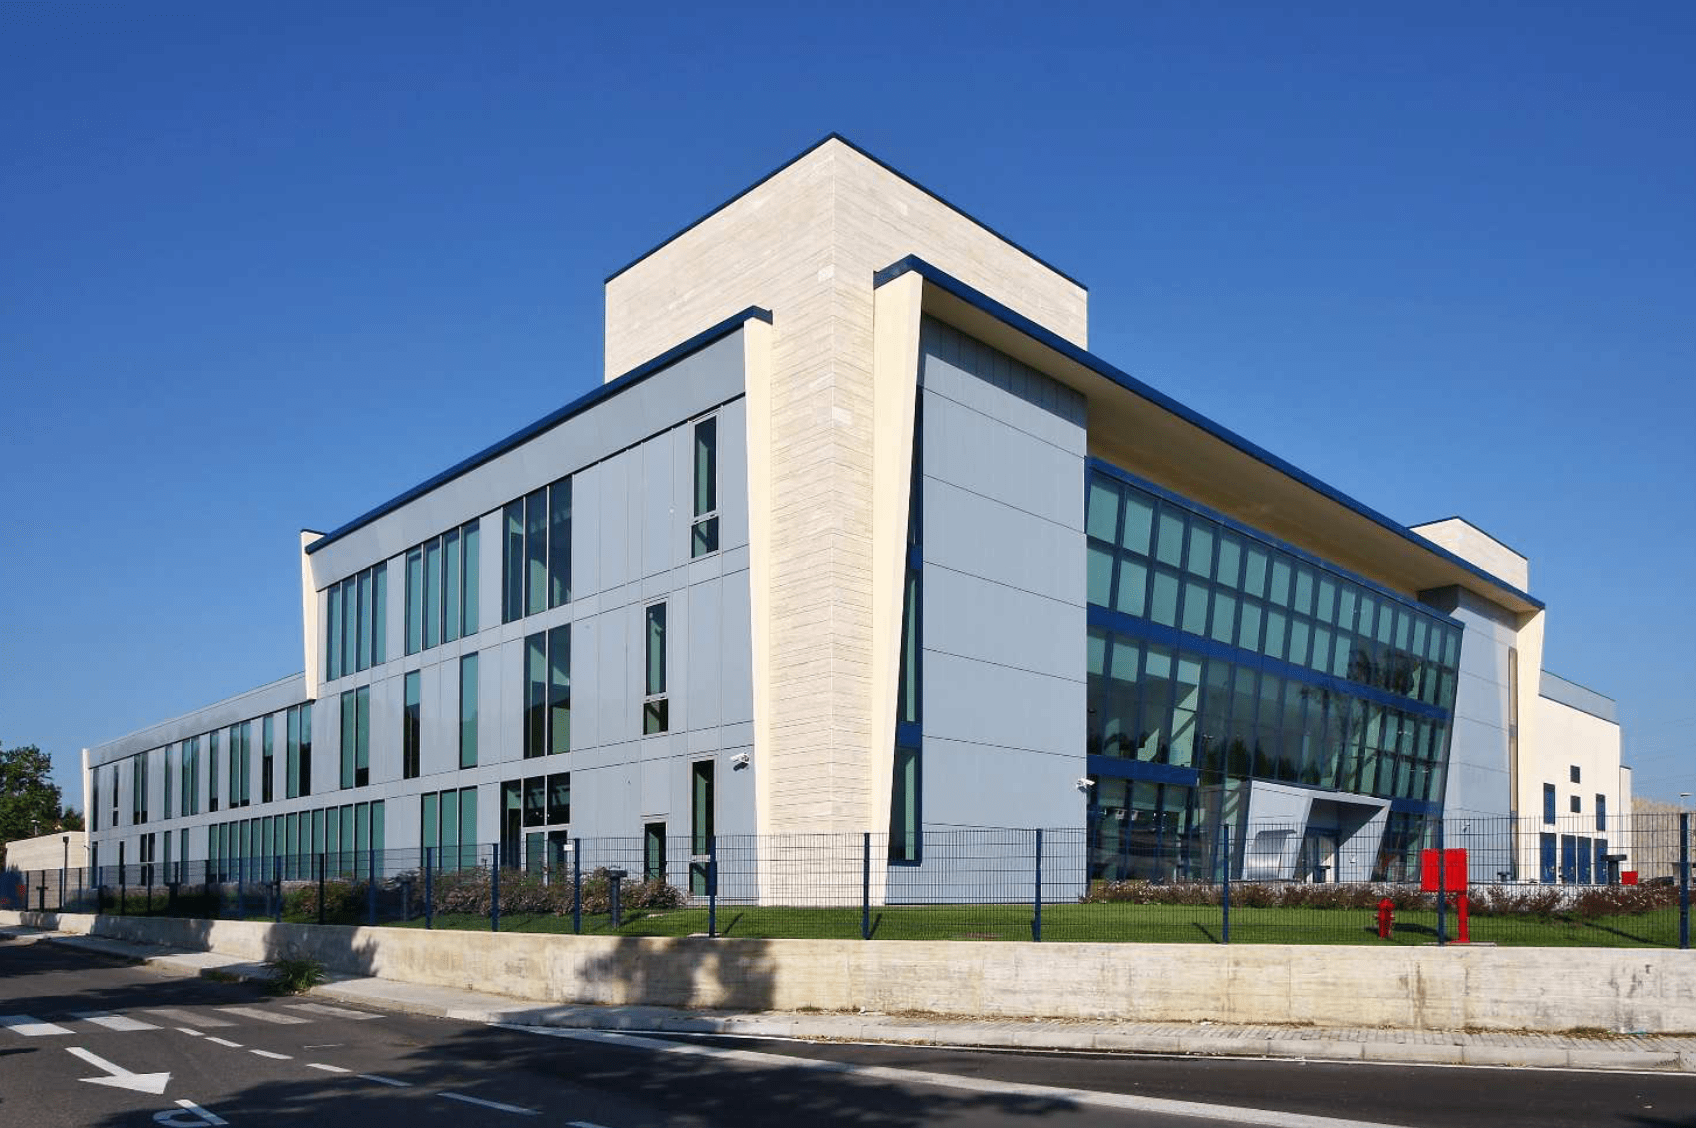
\includegraphics[width=.49\linewidth]{images/edificio_cnao.jpg}}\hfill
		\subfloat[Una delle sale di trattamento del CNAO. Il fascio è in grado di raggiungere il paziente sia dall'alto che da sinistra (cita
		%rivista asimmetrie, DOI 10.23801/asimmetrie.2023.35.03
		).]{\label{fig:sala_cnao}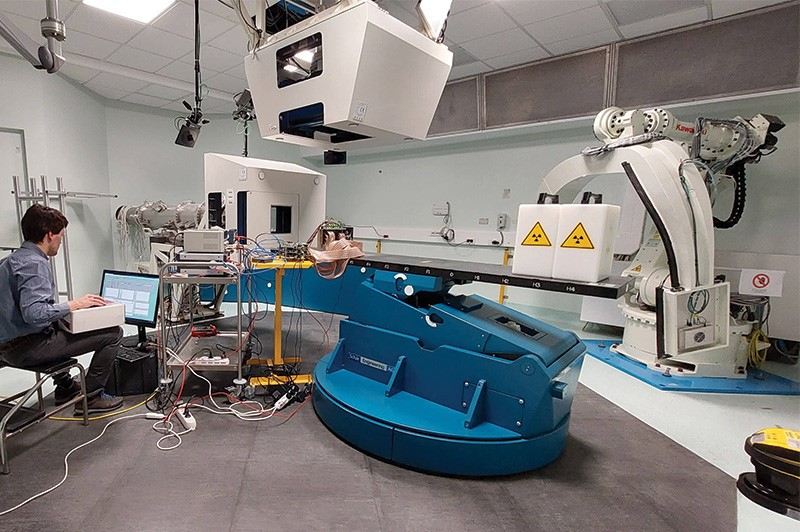
\includegraphics[width=.49\linewidth]{images/sala_cnao.jpg}}\par 
		\subfloat[Il sincrotrone del CNAO, situato in un bunker di $1600\mbox{ m}^2$ isolato dal resto della struttura con spesse pareti in cermento armato (cita
		%https://www.facebook.com/photo/?fbid=2533501746969553&set=a.1378679705785102
		).]{\label{fig:sincrotrone_cnao}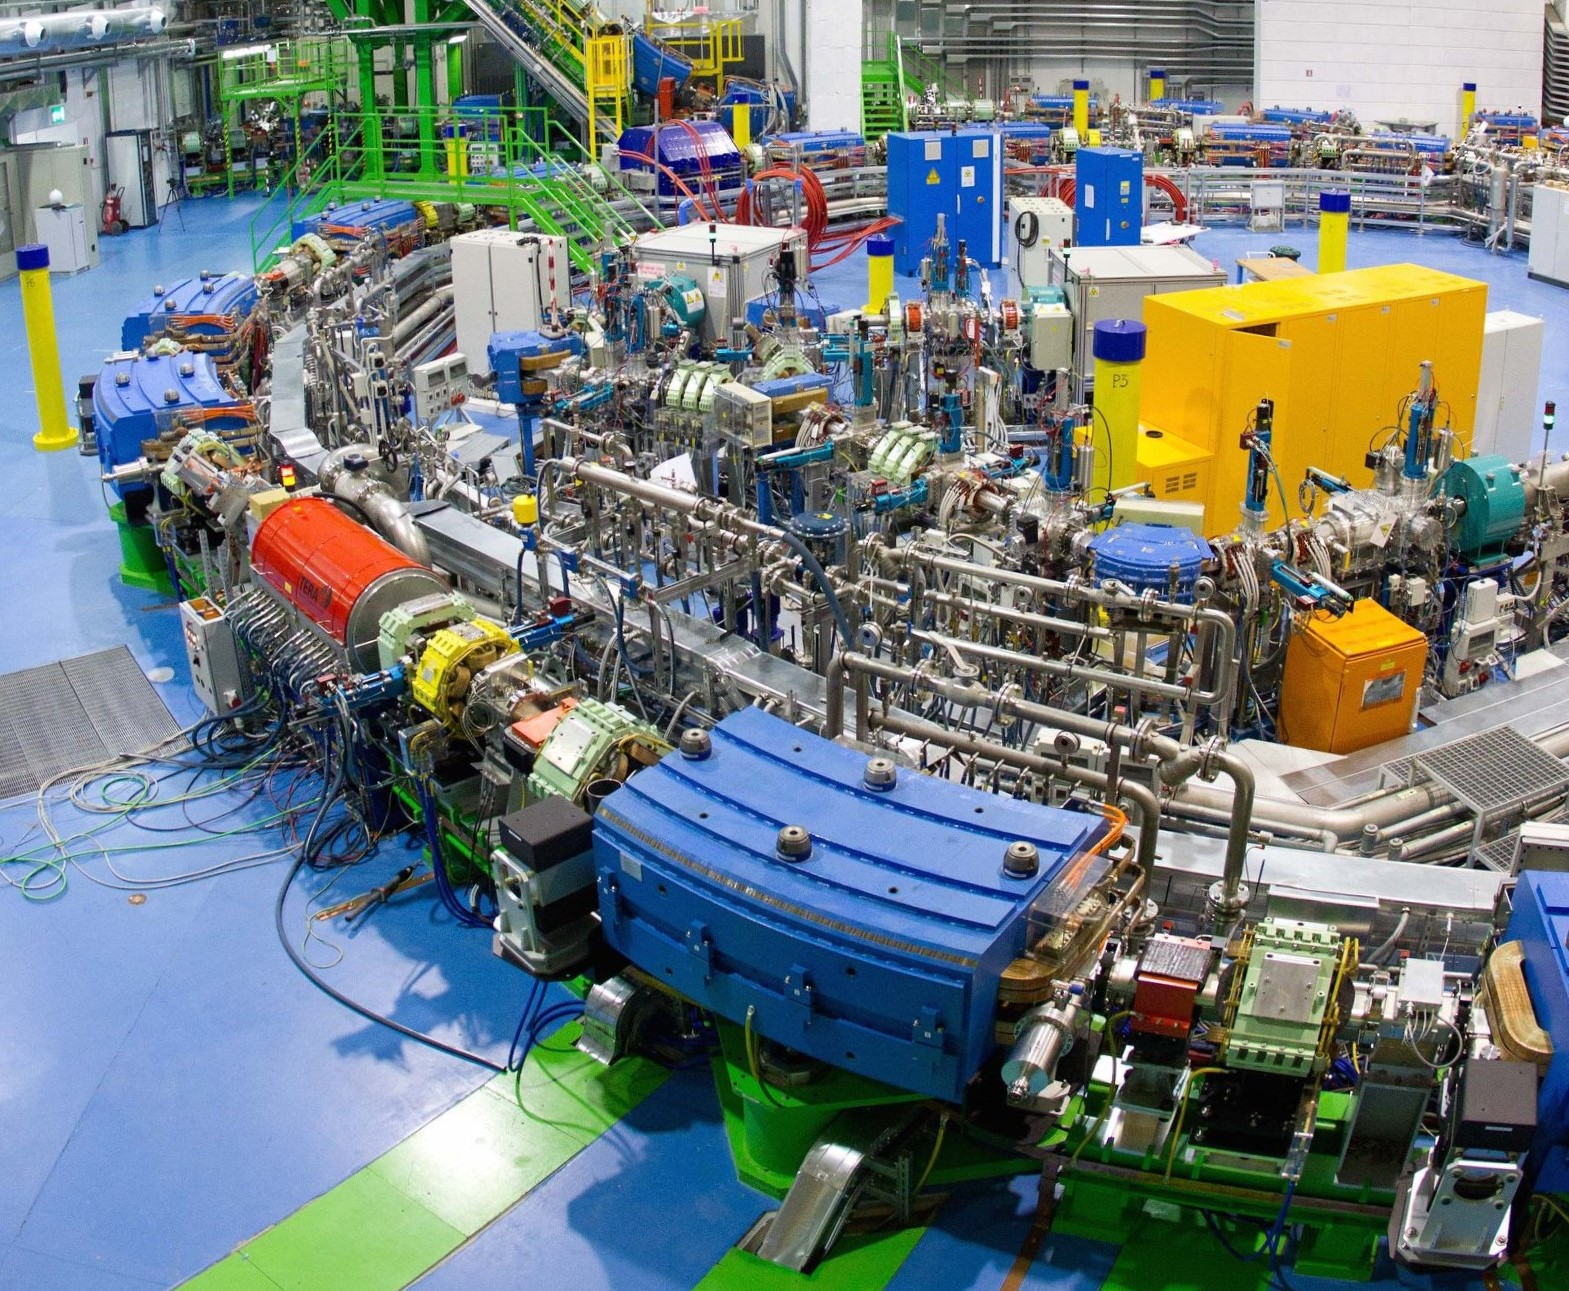
\includegraphics[width=.49\linewidth]{images/sincrotrone_cnao.jpg}}
		\caption{Immagini relative al CNAO di Pavia.}
		\label{fig:cnao}
	\end{figure}
	
	Il centro adroterapico italiano più recente è il Proton Therapy Center (PTC) di Trento, la cui attività clinica ha avuto inizio nell'ottobre del 2014 (cita
	%https://protonterapia.provincia.tn.it/eng
	). Il PCT, che è una delle unità operative del Dipartimento di Oncologia dell'Ospedale di Trento, utilizza solo fasci di protoni accelerati da un ciclotrone a un'energia di $70$--$226 \mbox{ MeV}$ (cita
	%trentoPCT.pdf
	). Uno dei punti di forza del PCT è la sua capacità di erogare protoni per mezzo di sistemi rotanti (gantry, \hyperref[fig:gantry]{Fig. 1.6}), garantendo un trattamento del paziente full-body a $360^\circ$ per patologie come tumori cerebrali e della base cranica, del distretto cervico-cefalico, della colonna vertebrale, sarcomi dei tessuti molli e tumori pediatrici (cita
	%https://www.apss.tn.it/Azienda/Unita-operative-e-strutture-organizzative/Unita-operativa-protonterapia-Trento#cosa_fa
	). Inoltre il centro adroterapico trentino è il primo in Italia a erogare un fascio di protoni in modalità attiva; quest'ultima, a differenza delle modalità uniforme e passiva, utilizza campi magnetici per deviare il percorso di ciascun fascio di protoni verso la posizione target, determinata subito prima che la dose venga erogata (cita	%https://www.radioterapiaitalia.it/wp-content/uploads/2017/03/Amichetti-Proton-parte-1.pdf
	,
	%https://www.ncbi.nlm.nih.gov/pmc/articles/PMC4651068/
	).
	
	\begin{figure}[H]
		\centering
		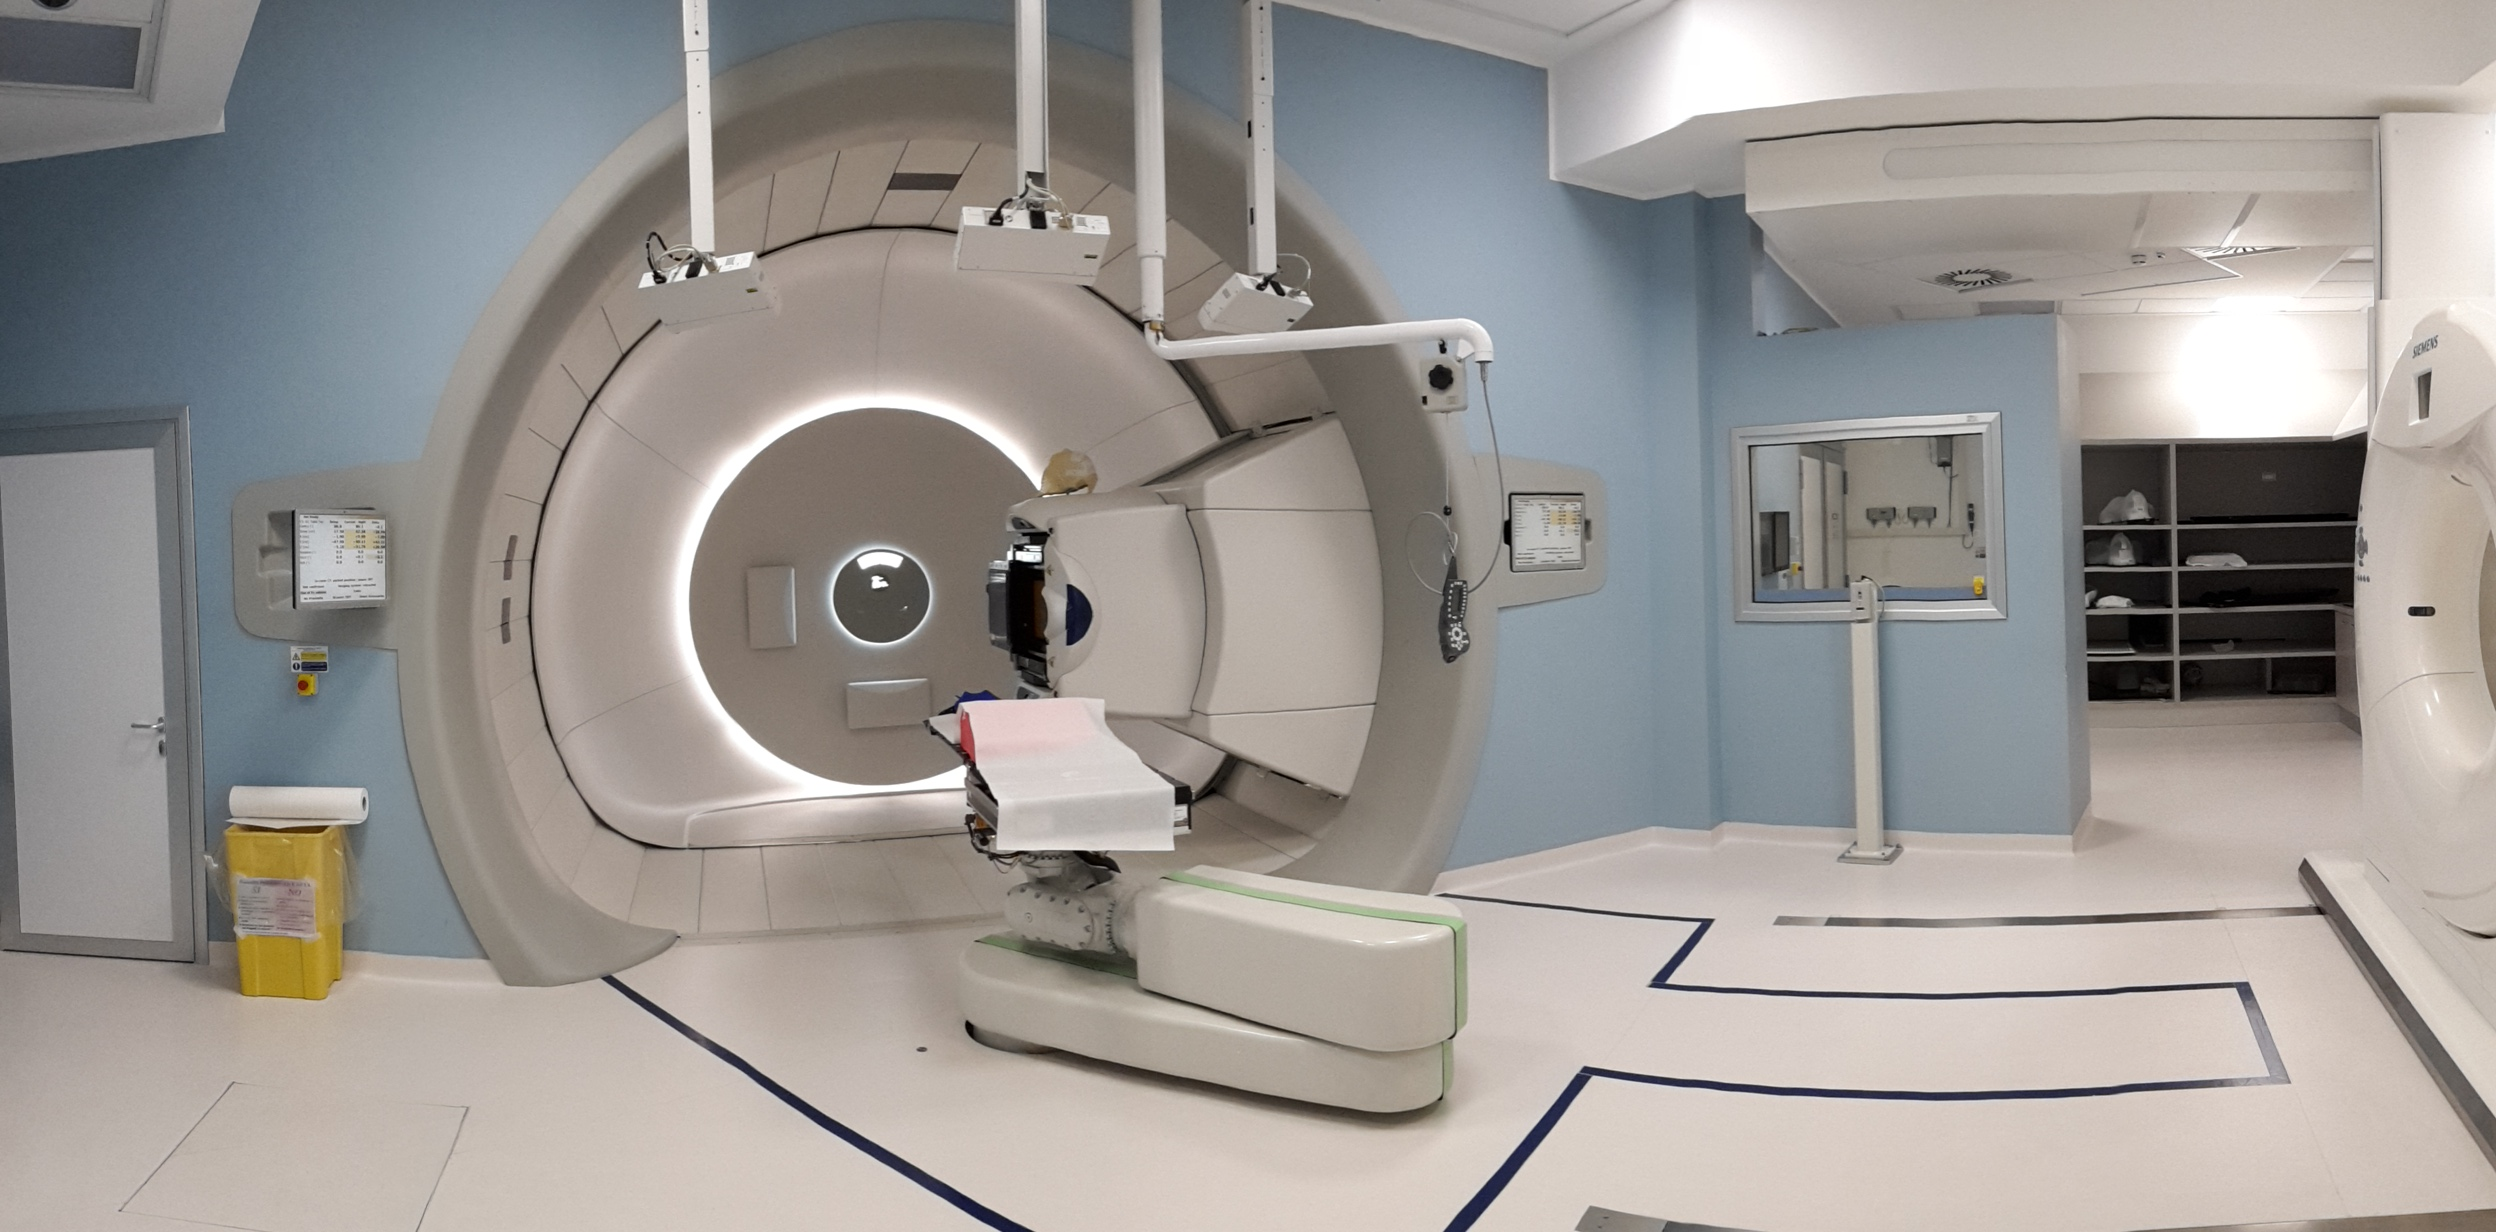
\includegraphics[width=0.9\linewidth]{images/gantry.jpg}
		\caption{Gantry Blu del Centro di Protonterapia di Trento (cita
			%https://it.wikipedia.org/wiki/Protonterapia
			).}
		\label{fig:gantry}
	\end{figure}
	
	Il PCT possiede due linee protoniche dedicate ai trattamenti clinici dotate di gantry e una linea fissa utilizzata per attività sperimentali di ricerca e sviluppo (R\&D). Le attività di R\&D non sono legate esclusivamente alla protonterapia ma anche a contesti lontani dall'ambito medico, per esempio gli ambiti aerospaziale con la radioprotezione (si veda \hyperref[label]{radioprotezione}) ed elettronico con lo studio di componenti elettroniche radioresistenti, l'analisi dei materiali e lo sviluppo di rivelatori (cita
	%https://protonterapia.provincia.tn.it/Per-i-ricercatori?/eng/switchlanguage/to/protonterapia_frontend/researchers
	). 
	
	\subsubsection{Sontorno radioterapia}
	Vogliamo ricordare che dietro ai trattamenti adroterapici ci sono varie tecniche di TAC, etc.
	treatment planning (TP)The Treatmenet Planning System
	TPS is the software that evaluate
	the machine parameters in order
	to obtain a dosimetric goal in the
	patient.
	oer esempio al cnao durata media di tot mesi per il trattamento , tot sedute
	che immobilizzano il paziente, non è un corpo rigido e quindi le sua proprietà dipendono dal tempo
	CT PET MRI
	\section{Effetti biologici della radiazione}
	
	
	
	
	
	
%	l’idea di usare i protoni per il trattamento del cancro fu proposta per la prima volta nel 1946 L’adroterapia è un forma molto avanzata di radioterapia. La radioterapia, da sola o associata a chirurgia e/o a chemioterapia, migliora il controllo locale in diverse patologie tumorali. Inoltre, la natura non invasiva delle radiazioni rappresenta una valida alternativa per quei tumori non aggredibili chirurgicamente perché localizzati in sedi anatomiche complicate da organi vitali o deputati a funzioni la cui asportazione sarebbe troppo invalidante per il paziente.
	
%	La forza dell’adroterapia è nelle proprietà fisiche e radiobiologiche uniche delle particelle cariche (adroni): esse possono penetrare nei tessuti con poca diffusione e depositare la massima energia appena prima di fermarsi. Ciò consente di definire in modo molto preciso la region da irradiare. La caratteristica forma a picco del deposito di energia è chiamata picco di Bragg ed è diventata il simbolo dell’adroterapia.

% dire che FOOT L'esperimento FOOT unisce laboratori giapponesi, tedeschi e italiani al ne di raccogliere dati fondamentali per migliorare la conoscenza delle interazioni tra i fasci adronici e il materiale

	
	
	
	
			
	
	\chapter*{Conclusioni}
		Let's cite! Einstein's journal paper \cite{einstein} and Dirac's book \cite{dirac} are physics-related items.
	\newpage	
	\printbibliography[
		heading=bibintoc,
		title={Bibliografia}
		]
		 	
\end{document}

